\documentclass[12pt]{article}

% packages

%\usepackage{times} % alt: cmbright
\usepackage[top=1in, bottom=1in, left=1in, right=1in]{geometry}
\usepackage{natbib}
\usepackage{amsmath}
\usepackage{amssymb}
\usepackage{latexsym}
\usepackage{sectsty}
\usepackage{amsfonts}
\usepackage{epsfig}
\usepackage{url}
\usepackage{microtype}
\usepackage{fixmath}
\usepackage{hyperref}
\usepackage{amsthm}
\usepackage{subfigure}
\usepackage{float}
\usepackage{hyperref}

\newtheorem{lem}{Lemma}
\newtheorem{defn}{Assumption}
\newtheorem{propty}{Property}
\newtheorem{thm}{Theorem}

% references

\newcommand{\mysec}[1]{Section~\ref{sec:#1}}
\newcommand{\myapp}[1]{Appendix~\ref{app:#1}}
\newcommand{\myeq}[1]{Equation~\ref{eq:#1}}
\newcommand{\myeqp}[1]{Eq.~\ref{eq:#1}}
\newcommand{\mychap}[1]{Chapter~\ref{chap:#1}}
\newcommand{\myfig}[1]{Figure~\ref{fig:#1}}

% math conveniences

\newcommand{\g}{\,\vert\,}
\newcommand{\E}{\textrm{E}}
\newcommand{\vct}[1]{\textbf{#1}}
\newcommand{\realline}{\mathbb{R}}
\newcommand{\indpt}{\protect\mathpalette{\protect\independenT}{\perp}}
\def\independenT#1#2{\mathrel{\rlap{$#1#2$}\mkern2mu{#1#2}}}
\newcommand{\h}[1]{\textrm{H}\left( #1 \right)}
\newcommand{\half}{\frac{1}{2}}
\newcommand{\new}{\textrm{new}}

\newcommand{\mult}{\textrm{Mult}}
\newcommand{\dir}{\textrm{Dir}}
\newcommand{\discrete}{\textrm{Discrete}}
\newcommand{\Bern}{\textrm{Bern}}
\newcommand{\DP}{\textrm{DP}}
\newcommand{\GP}{\textrm{GP}}
\newcommand{\Bet}{\textrm{Beta}}

% paragraph spacing

\setlength{\parindent}{0pt}
\setlength{\parskip}{2ex plus 0.5ex minus 0.2ex}

\allsectionsfont{\sffamily\mdseries}
\paragraphfont{\sffamily\bfseries}

\usepackage{algorithm}
\usepackage{algorithmic}
\renewcommand{\algorithmicrequire}{\textbf{Input:}}
\renewcommand{\algorithmicensure}{\textbf{Output:}}


\begin{document}

\title{\textsf{Diffusion Homework}}
\author{\textsf{Daqing Yi}}
\date{\textsf{CS670}}

\maketitle

\section{Introduction}

This lab aims trying diffusion models in different graph structures. Let $ x_{i} $ be the position in two dimensions of a node $ i $ and is randomly initialized. Experiments are taken to see position of nodes changes over time and the relevance with \emph{Fielder eigenvalue}.

\subsection{Problem Statement}

In a multi-agent system, the interaction relationship between agents is defined by graph topology, the graph Laplacian of which is denoted as $ L $. $ L $ is defined as $ L = D - A $, in which $ D $ is degree matrix of a graph and $ A $ is adjacency matrix of a graph. The position of each agent is influenced by the positions of other agents. The influence is defined by a diffusion model. In this lab, the position of an agent is two dimension. The motion in each dimension is independent with the motion in the other dimension. Let $ \mathbf{x} $ be a vector representing the positions of all agents in the system, the diffusion model can be written as:

\begin{equation}
\dot{\mathbf{x}}(t) = - L \mathbf{x(t)}.
\end{equation}

Simulating this process in discrete steps, we use
\begin{equation}
\begin{aligned}
\mathbf{v}_{t} & = - L \mathbf{x}_{t}, \\
\mathbf{x}_{t+\Delta t} & = \mathbf{x}_{t} + \mathbf{v}_{k+1} * \Delta t.
\end{aligned}
\end{equation}

The results and analyses in five cases are given in next section.

\section{Case study}

\subsection{A connected graph with 2 nodes}

The topology is given in Fig.\ref{fig:C1}. 
\begin{figure}[htbp]
\centering
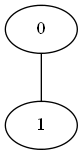
\includegraphics[width=0.08\textwidth]{./C1}
\caption{A connected graph with 2 nodes}
\label{fig:C1}
\end{figure}


\paragraph{\textbf{Graph Laplacian:}}

$
L = 
\begin{bmatrix}
1 & -1 \\
-1 & 1
\end{bmatrix}
$

\paragraph{\textbf{Eigenvalues:}}

$
\lambda = 
\begin{bmatrix}
0 & 2 
\end{bmatrix}
$

\begin{figure}[htbp]
\centering
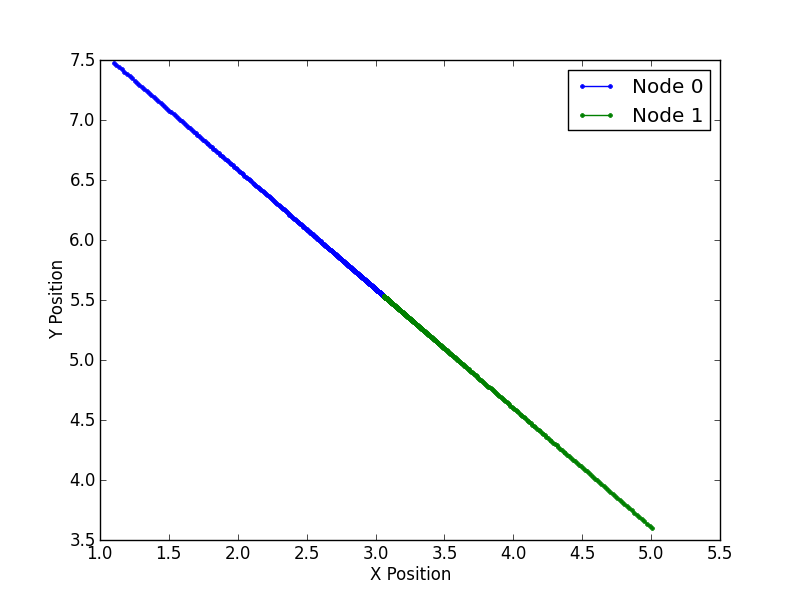
\includegraphics[width=0.4\textwidth]{./C1_mo}
\caption{Nodes motion of a connected graph with 2 nodes}
\label{fig:C1_mo}
\end{figure}

\begin{figure}[tbp]
\centering
\caption{\label{fig:C1_dyno}Velocities and positions in X and Y of a connected graph with 2 nodes.}

\subfigure[Velocity in X]
{
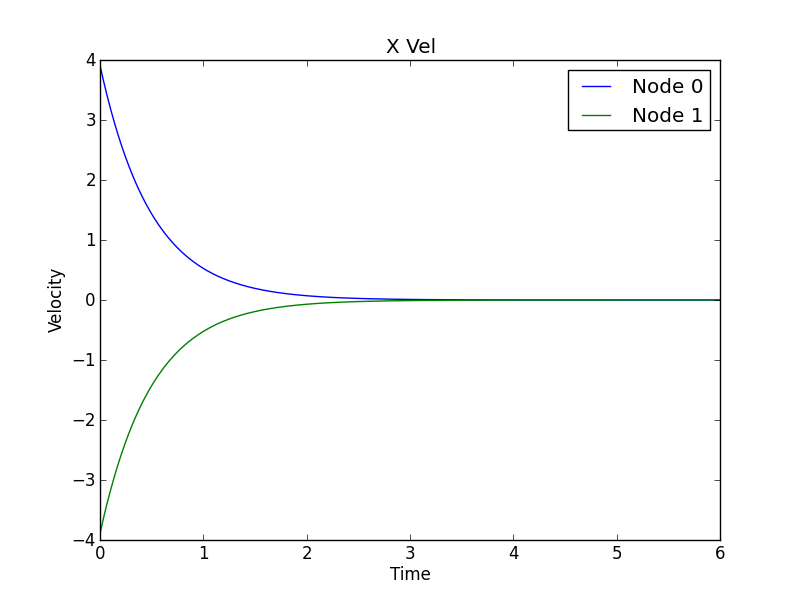
\includegraphics[width=0.4\textwidth]{./C1_velX}
\label{fig:C1_velX}
}
%\mbox{\hspace{0.5cm}}
\subfigure[Velocity in Y]
{
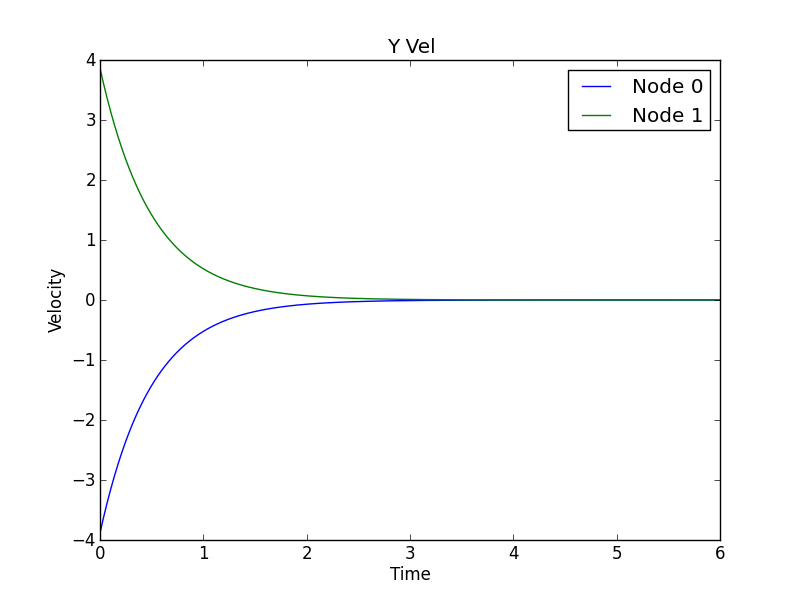
\includegraphics[width=0.4\textwidth]{./C1_velY}
\label{fig:C1_velY}
}
\\
\subfigure[Position in X]
{
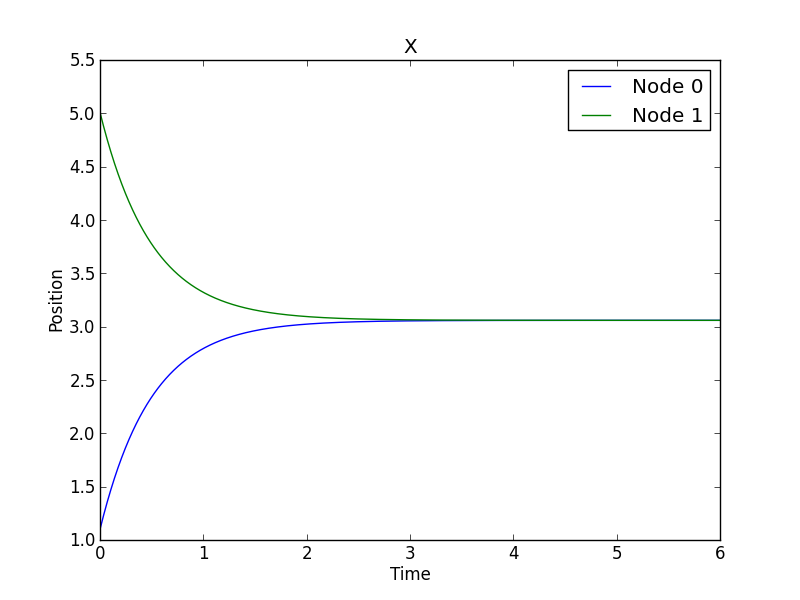
\includegraphics[width=0.4\textwidth]{./C1_posX}
\label{fig:C1_posX}
}
%\mbox{\hspace{0.5cm}}
\subfigure[Position in Y]
{
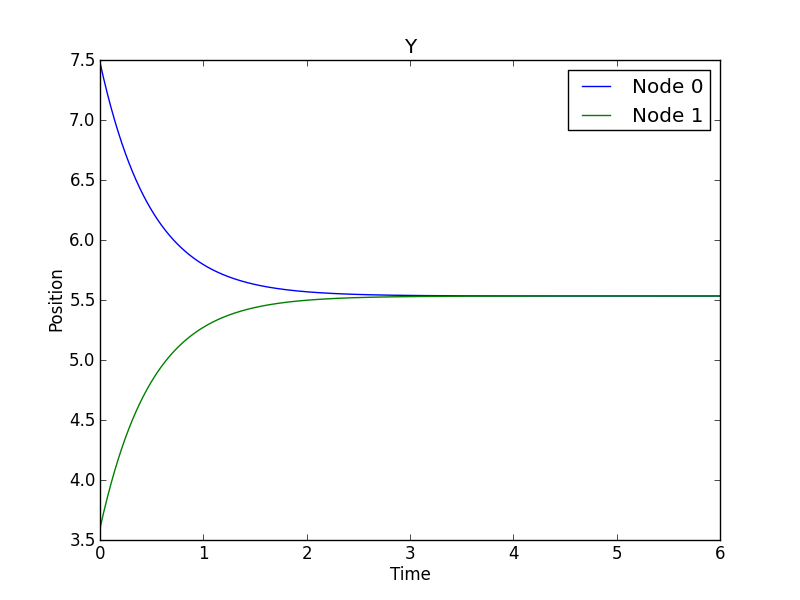
\includegraphics[width=0.4\textwidth]{./C1_posY}
\label{fig:C1_posY}
}
\end{figure}


\subsection{A fully connected graph with 4 nodes}

The topology is given in Fig.\ref{fig:C2}. 
\begin{figure}[htbp]
\centering
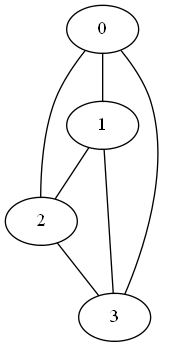
\includegraphics[width=0.1\textwidth]{./C2}
\caption{A fully connected graph with 4 nodes}
\label{fig:C2}
\end{figure}

\paragraph{\textbf{Graph Laplacian:}}

$
L = 
\begin{bmatrix}
3 & -1 & -1 & -1 \\
-1 & 3 & -1 & -1 \\
-1 & -1 & 3 & -1 \\
-1 & -1 & -1 & 3 
\end{bmatrix}
$

\paragraph{\textbf{Eigenvalues:}}

$
\lambda = 
\begin{bmatrix}
0 & 4 & 4 & 4
\end{bmatrix}
$

\begin{figure}[htbp]
\centering
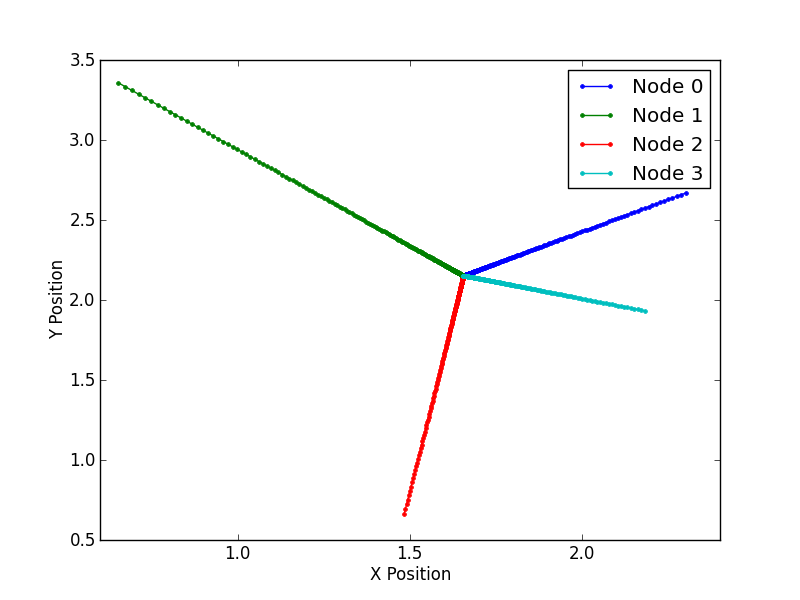
\includegraphics[width=0.4\textwidth]{./C2_mo}
\caption{Nodes motion of a fully connected graph with 4 nodes}
\label{fig:C2_mo}
\end{figure}

\begin{figure}[tbp]
\centering
\caption{\label{fig:C2_dyno}Velocities and positions in X and Y of a fully connected graph with 4 nodes.}

\subfigure[Velocity in X]
{
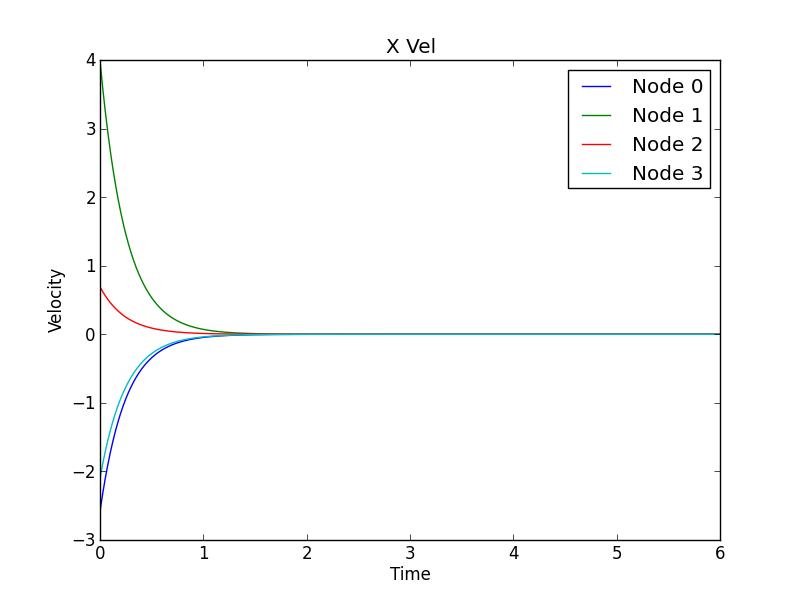
\includegraphics[width=0.4\textwidth]{./C2_velX}
\label{fig:C2_velX}
}
%\mbox{\hspace{0.5cm}}
\subfigure[Velocity in Y]
{
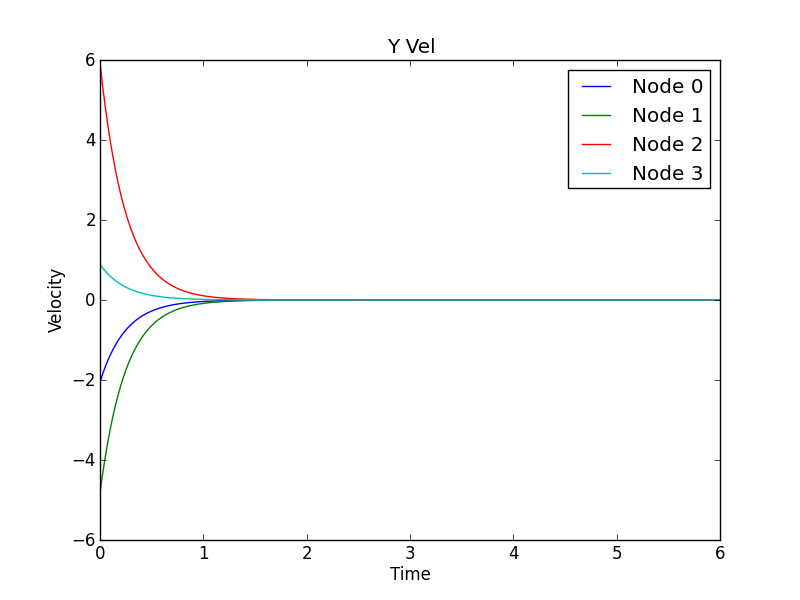
\includegraphics[width=0.4\textwidth]{./C2_velY}
\label{fig:C2_velY}
}
\\
\subfigure[Position in X]
{
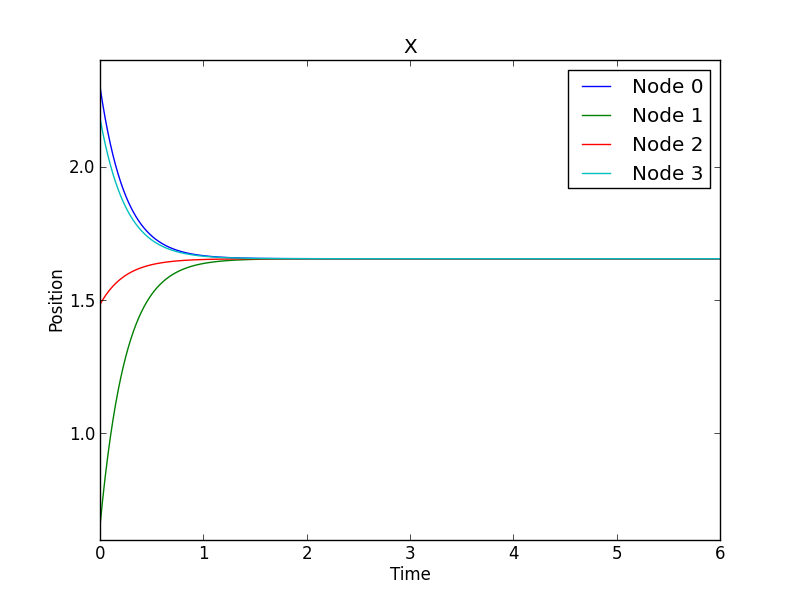
\includegraphics[width=0.4\textwidth]{./C2_posX}
\label{fig:C2_posX}
}
%\mbox{\hspace{0.5cm}}
\subfigure[Position in Y]
{
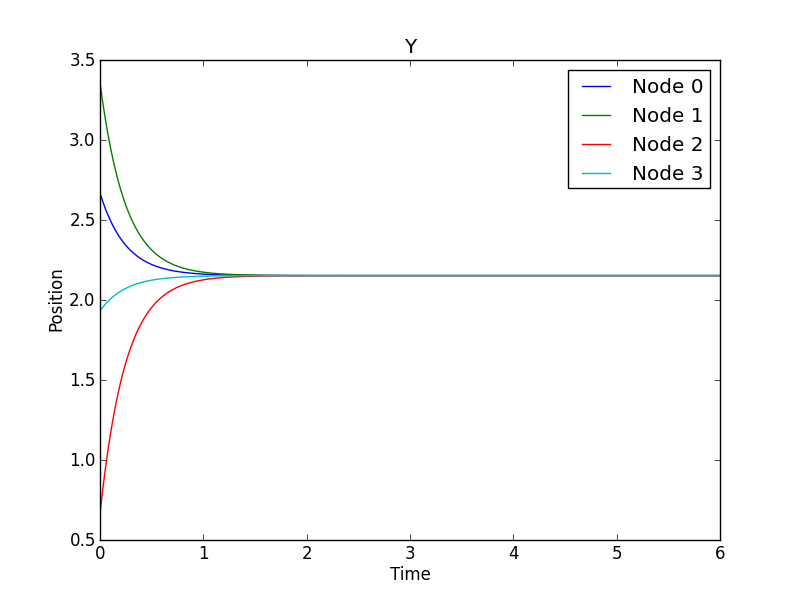
\includegraphics[width=0.4\textwidth]{./C2_posY}
\label{fig:C2_posY}
}
\end{figure}

\subsection{A ring graph with 5 nodes}

The topology is given in Fig.\ref{fig:C3}. 
\begin{figure}[htbp]
\centering
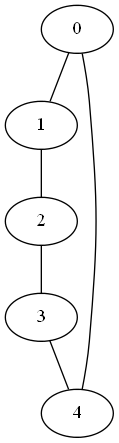
\includegraphics[width=0.1\textwidth]{./C3}
\caption{A ring graph with 5 nodes}
\label{fig:C3}
\end{figure}

\paragraph{\textbf{Graph Laplacian:}}

$
L = 
\begin{bmatrix}
2 & -1 & 0 & 0 & -1 \\
-1 & 2 & -1 & 0 & 0 \\
0 & -1 & 2 & -1 & 0 \\
0 & 0 & -1 & 2 & -1 \\
-1 & 0 & 0 & -1 & 2 
\end{bmatrix}
$

\paragraph{\textbf{Eigenvalues:}}

$
\lambda = 
\begin{bmatrix}
0 & 1.382 & 1.382 & 3.618 & 3.618
\end{bmatrix}
$

\begin{figure}[htbp]
\centering
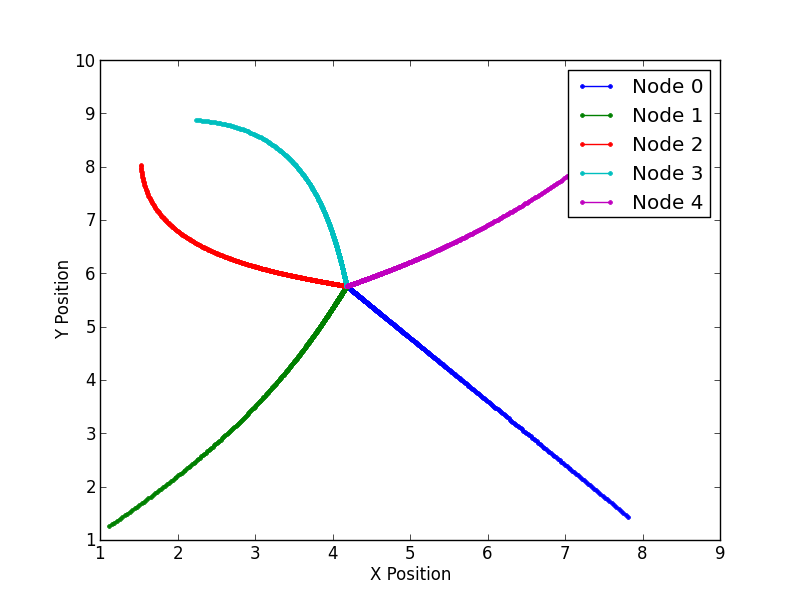
\includegraphics[width=0.4\textwidth]{./C3_mo}
\caption{Nodes motion of a ring graph with 5 nodes}
\label{fig:C3_mo}
\end{figure}

\begin{figure}[tbp]
\centering
\caption{\label{fig:C3_dyno}Velocities and positions in X and Y of a ring graph with 5 nodes.}

\subfigure[Velocity in X]
{
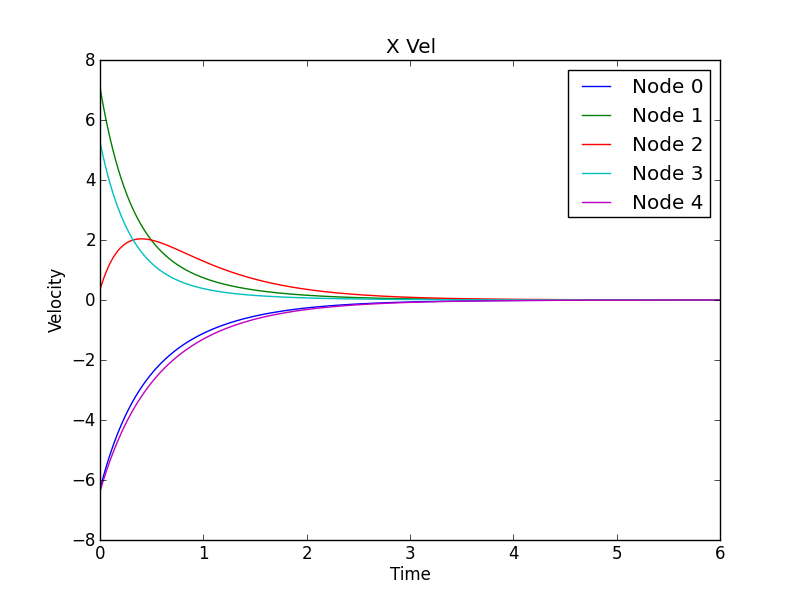
\includegraphics[width=0.4\textwidth]{./C3_velX}
\label{fig:C3_velX}
}
%\mbox{\hspace{0.5cm}}
\subfigure[Velocity in Y]
{
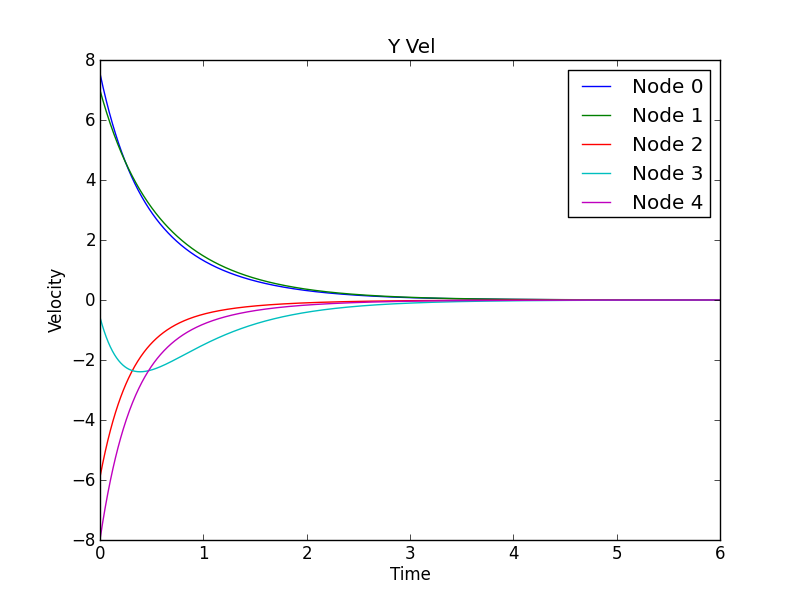
\includegraphics[width=0.4\textwidth]{./C3_velY}
\label{fig:C3_velY}
}
\\
\subfigure[Position in X]
{
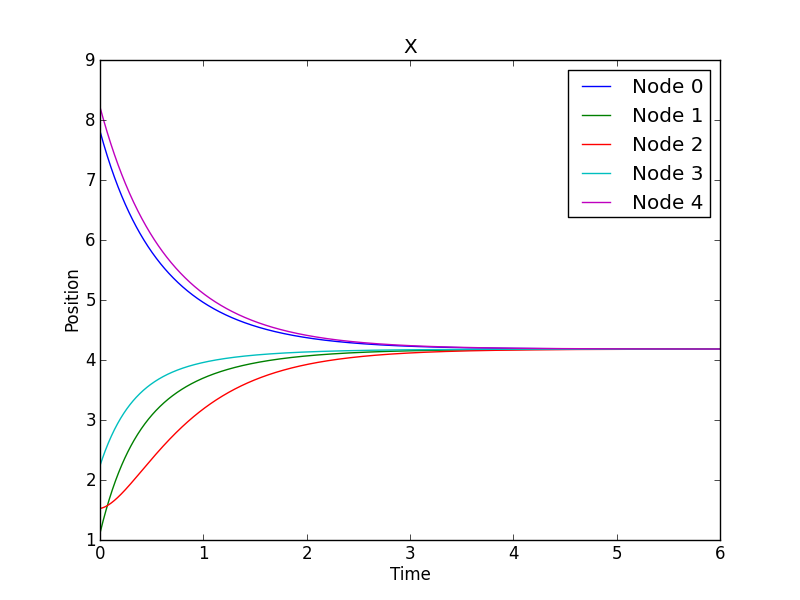
\includegraphics[width=0.4\textwidth]{./C3_posX}
\label{fig:C3_posX}
}
%\mbox{\hspace{0.5cm}}
\subfigure[Position in Y]
{
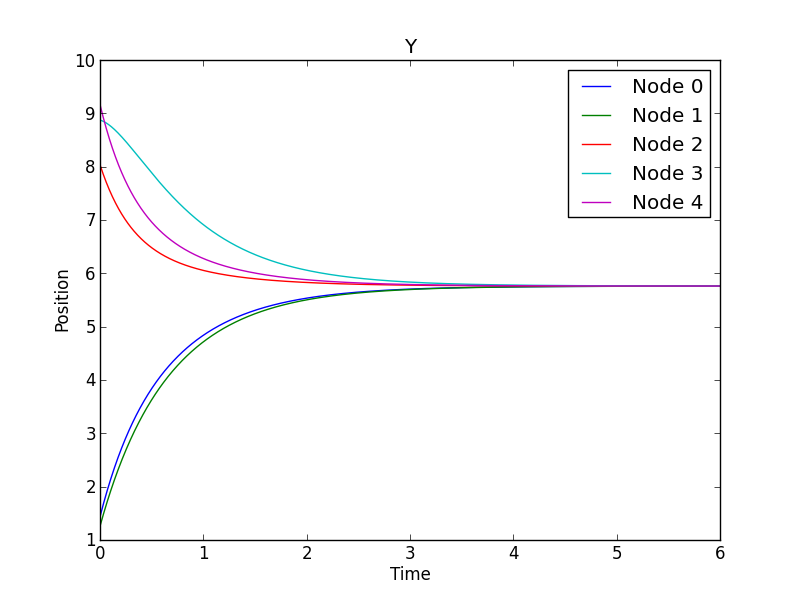
\includegraphics[width=0.4\textwidth]{./C3_posY}
\label{fig:C3_posY}
}
\end{figure}

\subsection{A random graph with 10 nodes}

The topology is given in Fig.\ref{fig:C4}. 
\begin{figure}[htbp]
\centering
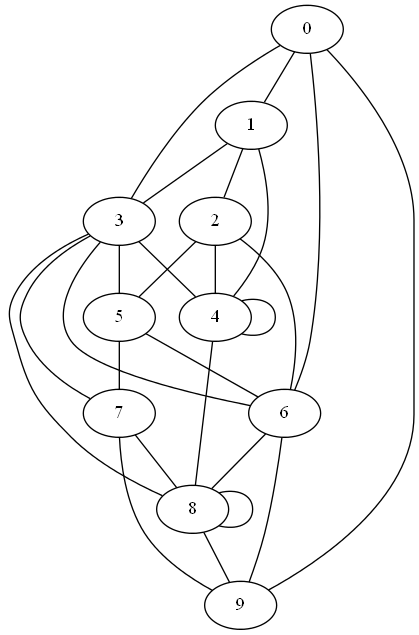
\includegraphics[width=0.6\textwidth]{./C4}
\caption{A random graph with 10 nodes}
\label{fig:C4}
\end{figure}

\paragraph{\textbf{Graph Laplacian:}}

$
L = 
\begin{bmatrix}
4 & -1 & 0 & -1 & 0 & 0 & -1 & 0 & 0 & -1 \\
-1 & 4 & -1 & -1 & -1 & 0 & 0 & 0 & 0 & 0 \\
0 & -1 & 4 & 0 & -1 & -1 & -1 & 0 & 0 & 0 \\
-1 & -1 & 0 & 7 & -1 & -1 & -1 & -1 & -1 & 0 \\
0 & -1 & -1 & -1 & 4 & 0 & 0 & 0 & -1 & 0 \\
0 & 0 & -1 & -1 & 0 & 4 & -1 & -1 & 0 & 0 \\
-1 & 0 & -1 & -1 & 0 & -1 & 6 & 0 & -1 & -1 \\
0 & 0 & 0 & -1 & 0 & -1 & 0 & 4 & -1 & -1 \\
0 & 0 & 0 & -1 & -1 & 0 & -1 & -1 & 5 & -1 \\
-1 & 0 & 0 & 0 & 0 & 0 & -1 & -1 & -1 & 4 \\
\end{bmatrix}
$

\paragraph{\textbf{Eigenvalues:}}

$
\lambda =  \\
\begin{bmatrix}
0.0 &   2.307 &   3.0  &   3.570  &  4.38087539 &  5.0 &  5.919 &   6.0 &   7.401 &   8.422
\end{bmatrix} 
$

\begin{figure}[htbp]
\centering
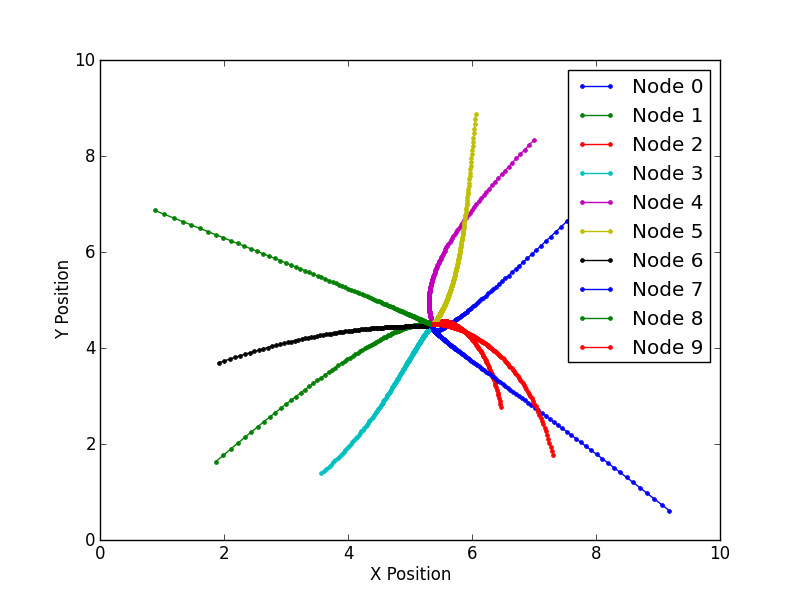
\includegraphics[width=0.4\textwidth]{./C4_mo}
\caption{Nodes motion of a random graph with 10 nodes}
\label{fig:C4_mo}
\end{figure}

\begin{figure}[tbp]
\centering
\caption{\label{fig:C4_dyno}Velocities and positions in X and Y of a random graph with 10 nodes.}

\subfigure[Velocity in X]
{
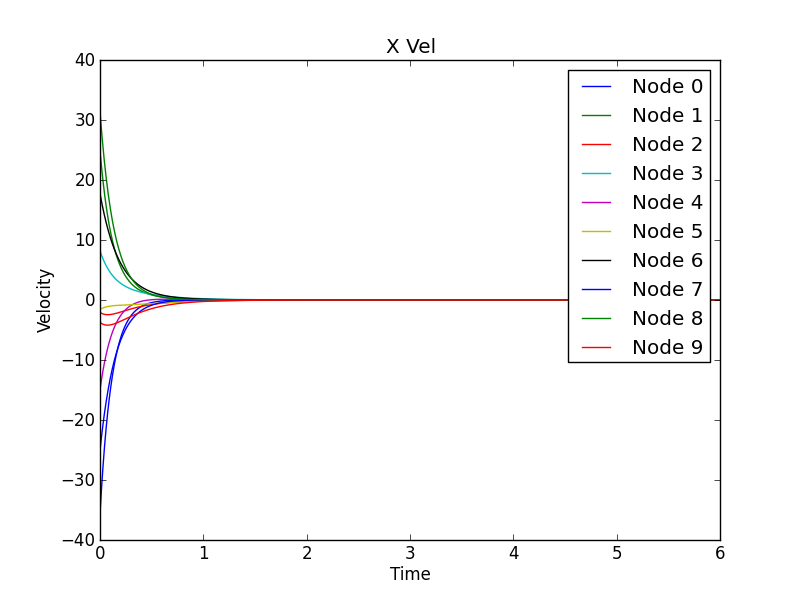
\includegraphics[width=0.4\textwidth]{./C4_velX}
\label{fig:C4_velX}
}
%\mbox{\hspace{0.5cm}}
\subfigure[Velocity in Y]
{
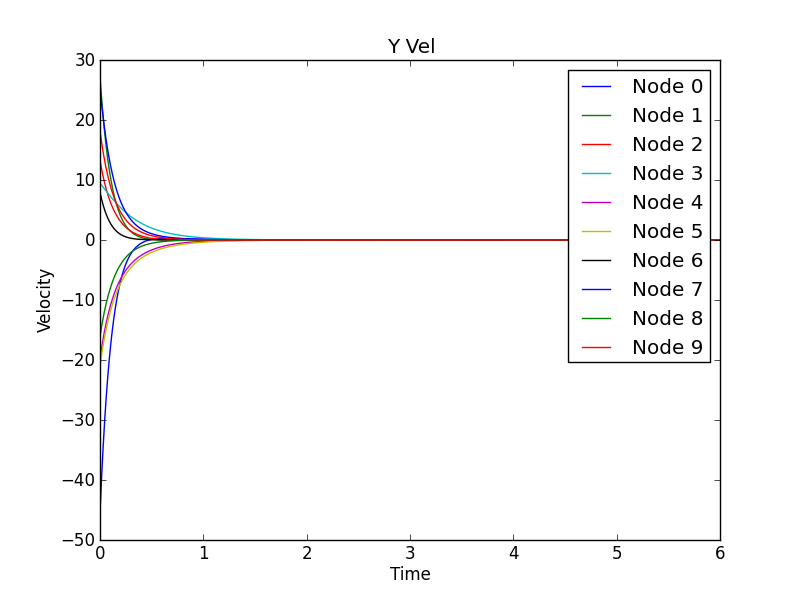
\includegraphics[width=0.4\textwidth]{./C4_velY}
\label{fig:C4_velY}
}
\\
\subfigure[Position in X]
{
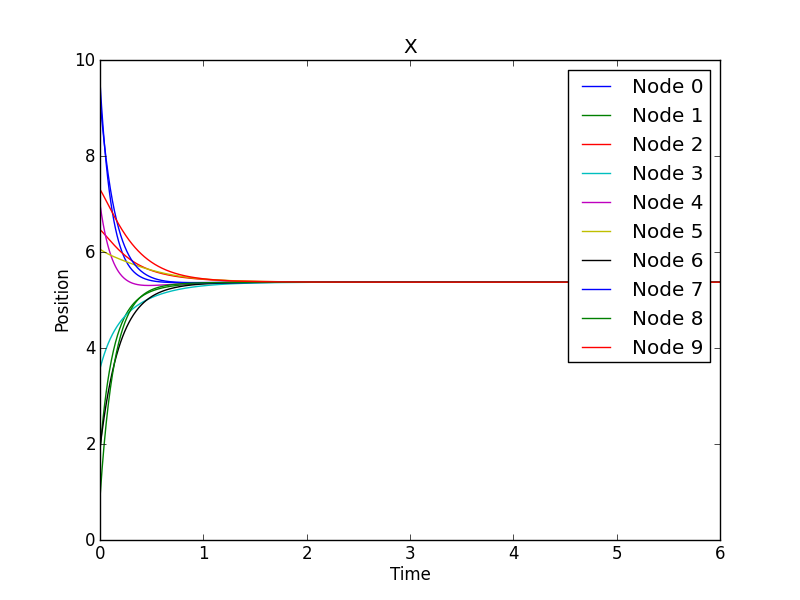
\includegraphics[width=0.4\textwidth]{./C4_posX}
\label{fig:C4_posX}
}
%\mbox{\hspace{0.5cm}}
\subfigure[Position in Y]
{
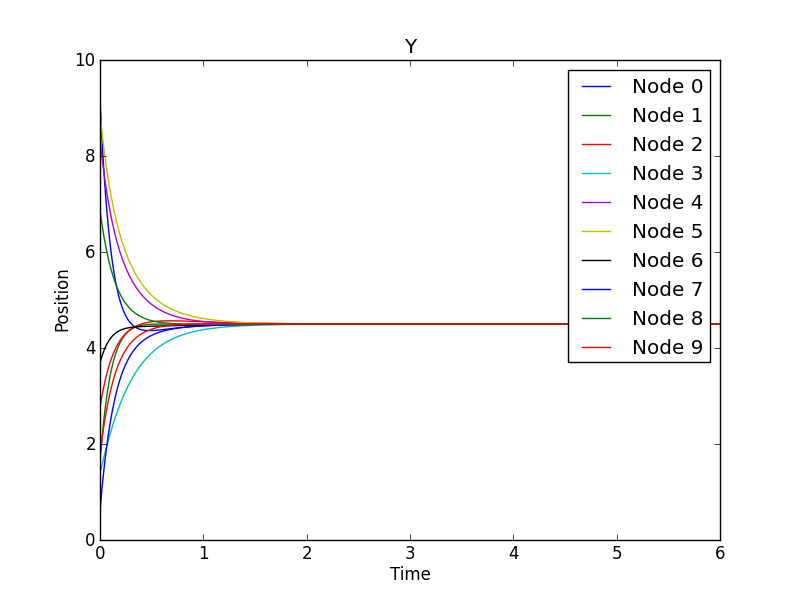
\includegraphics[width=0.4\textwidth]{./C4_posY}
\label{fig:C4_posY}
}
\end{figure}

\subsection{A graph with 8 nodes and 2 connected components}

The topology is given in Fig.\ref{fig:C5}. 
\begin{figure}[htbp]
\centering
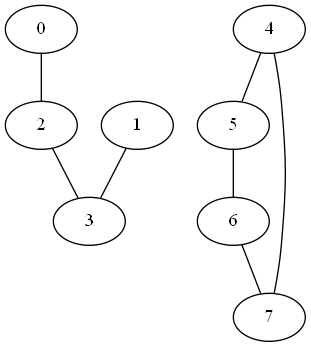
\includegraphics[width=0.4\textwidth]{./C5}
\caption{A graph with 8 nodes and 2 connected components}
\label{fig:C5}
\end{figure}

\paragraph{\textbf{Graph Laplacian:}}

$
L = 
\begin{bmatrix}
1 & 0 & -1 & 0 & 0 & 0 & 0 & 0 \\
0 & 1 & 0 & -1 & 0 & 0 & 0 & 0 \\
-1 & 0 & 2 & -1 & 0 & 0 & 0 & 0 \\
0 & -1 & -1 & 2 & 0 & 0 & 0 & 0 \\
0 & 0 & 0 & 0 & 2 & -1 & 0 & -1 \\
0 & 0 & 0 & 0 & -1 & 2 & -1 & 0 \\
0 & 0 & 0 & 0 & 0 & -1 & 2 & -1 \\
0 & 0 & 0 & 0 & -1 & 0 & -1 & 2 \\

\end{bmatrix}
$

\paragraph{\textbf{Eigenvalues:}}

$
\lambda = 
\begin{bmatrix}
0.0 & 0.0 & 0.586 & 2.0 & 2.0 & 2.0 & 3.414 & 4.0 
\end{bmatrix}
$

\begin{figure}[htbp]
\centering
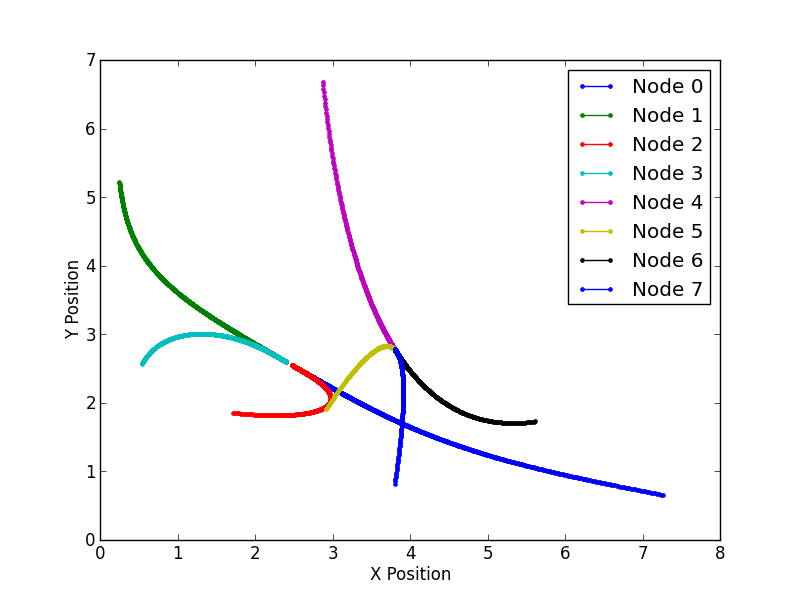
\includegraphics[width=0.4\textwidth]{./C5_mo}
\caption{Nodes motion of a graph with 8 nodes and 2 connected components.}
\label{fig:C5_mo}
\end{figure}

\begin{figure}[tbp]
\centering
\caption{\label{fig:C5_dyno}Velocities and positions in X and Y of a graph with 8 nodes and 2 connected components.}

\subfigure[Velocity in X]
{
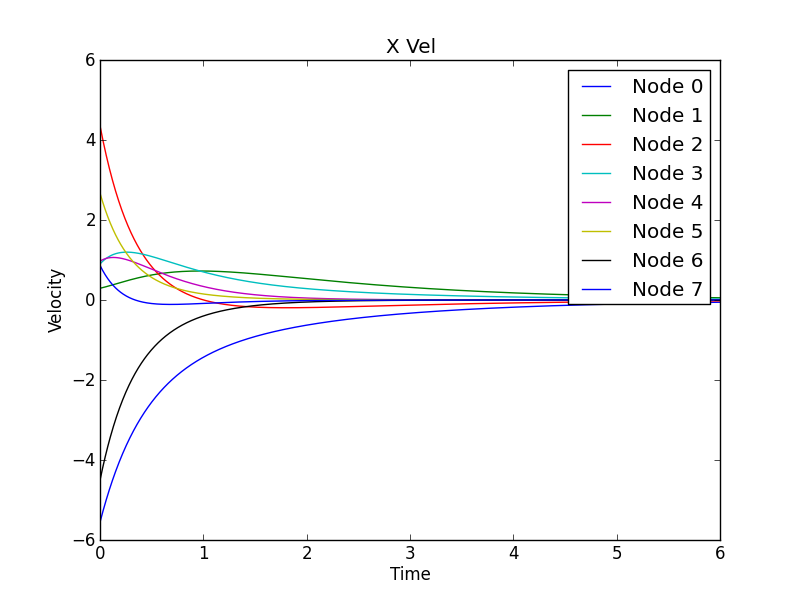
\includegraphics[width=0.4\textwidth]{./C5_velX}
\label{fig:C5_velX}
}
%\mbox{\hspace{0.5cm}}
\subfigure[Velocity in Y]
{
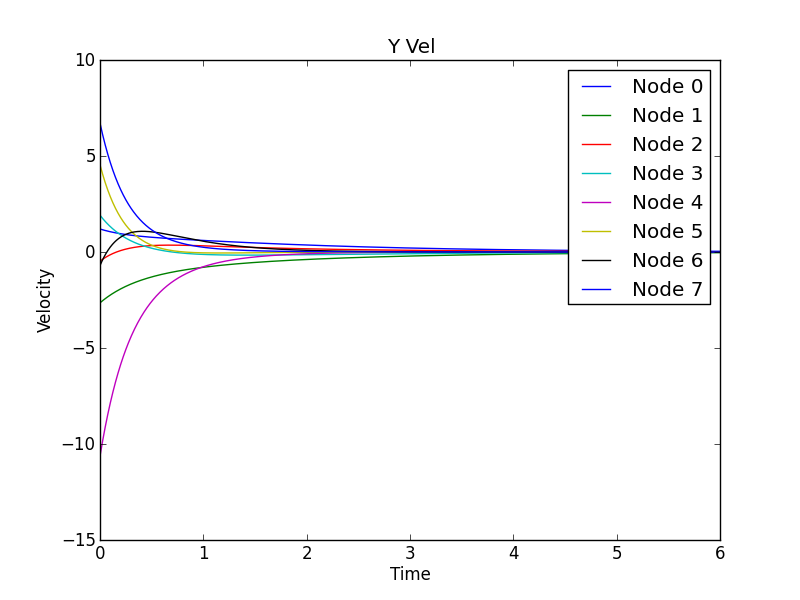
\includegraphics[width=0.4\textwidth]{./C5_velY}
\label{fig:C5_velY}
}
\\
\subfigure[Position in X]
{
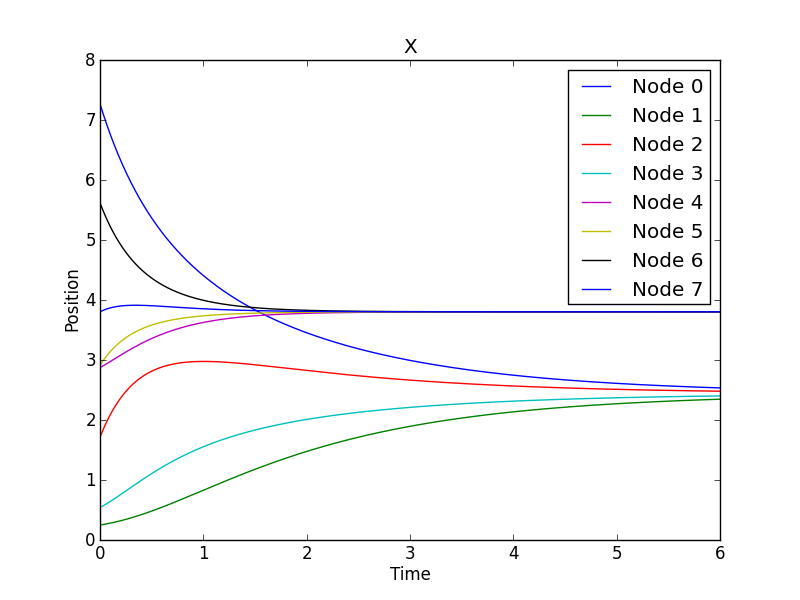
\includegraphics[width=0.4\textwidth]{./C5_posX}
\label{fig:C5_posX}
}
%\mbox{\hspace{0.5cm}}
\subfigure[Position in Y]
{
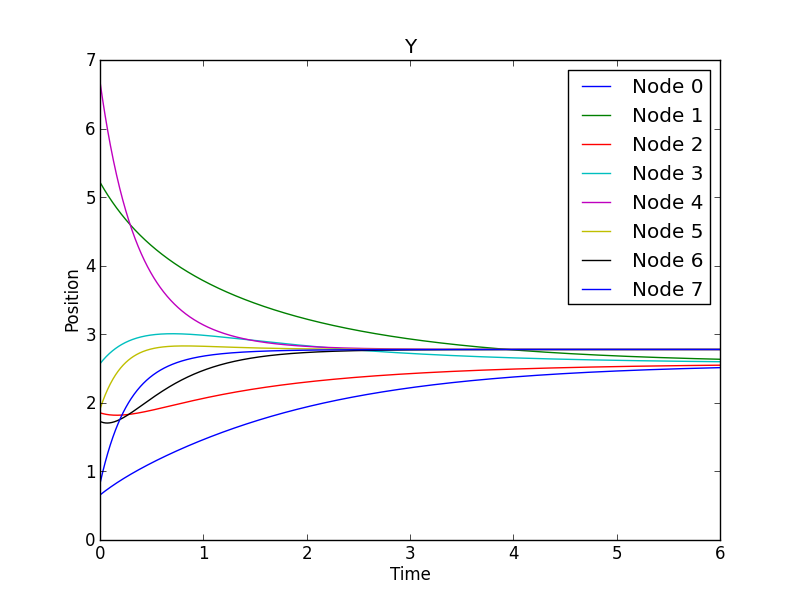
\includegraphics[width=0.4\textwidth]{./C5_posY}
\label{fig:C5_posY}
}
\end{figure}

\section{Discussion}

The eigenvalues in five cases are all positive, so all the node motion converges to centroid of initial positions. At the same time, the velocities all converge to zero. It is noticeable that in case 5, because there are two unconnected subgraphs, nodes converged into two positions separately, which is still decided by the centroid of initial positions in all nodes in each subgraph. 

\begin{tabular}{|c|c|}
\hline
case & Fieder eigenvalue \\\hline
1 & 2 \\\hline
2 & 4 \\\hline
3 & 1.382 \\\hline
4 & 2.307 \\\hline
5 & 0.586 \\\hline
\end{tabular}

\begin{figure}[htbp]
\centering
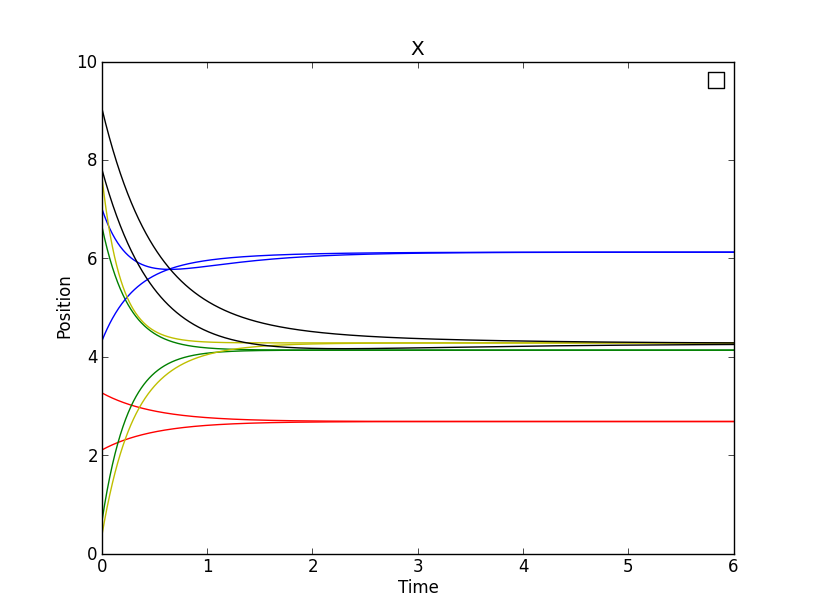
\includegraphics[width=0.5\textwidth]{./compare}
\caption{Case 1: red line, Case 2: green line, Case 3: blue line, Case 4: yellow line, Case 5: black line}
\label{fig:compare}
\end{figure}

I can see that case 5 has the smallest Fieder eignenvalue, the convergence of which is the slowest. While case 2, which has the biggest Fieder eigenvalue, has the highest convergence speed. It is obvious that the Fieder eigenvalue determines the connectivity of a graph, and it has an influence on the convergence speed.

\end{document}
